\documentclass[11pt,a4paper]{article}
\usepackage[T1]{fontenc}
\usepackage{lmodern}
\usepackage[spanish]{babel}
\usepackage[margin=2.5cm]{geometry}
\usepackage{graphicx}
\usepackage{amsmath}
\usepackage{booktabs}
\usepackage{tikz}
\usetikzlibrary{positioning,arrows.meta}
\usepackage{listings}
\lstset{basicstyle=\ttfamily\small,breaklines=true,frame=single,columns=fullflexible}
\usepackage[hidelinks]{hyperref}
\usepackage[backend=biber,style=ieee]{biblatex}
\addbibresource{referencias.bib}

\begin{document}
% Carátula del informe. Aporte de Angello Mendoza Bermello.
\begin{titlepage}
\centering
\thispagestyle{empty}

{\large\bfseries UNIVERSIDAD TÉCNICA ESTATAL DE QUEVEDO\par}
\vspace{0.3cm}
{\bfseries FACULTAD DE CIENCIAS DE LA COMPUTACIÓN Y DISEÑO DIGITAL\par}
\vspace{0.2cm}
{\bfseries CARRERA DE INGENIERÍA EN SOFTWARE\par}

\vspace{1.6cm}

{\bfseries ASIGNATURA\par}
{Sistemas Distribuidos\par}

\vspace{1.4cm}

{\Large\bfseries COMUNICACIÓN ENTRE PROCESOS DISTRIBUIDOS\\[0.2cm]
CON SOCKETS TCP Y gRPC\par}

\vspace{0.6cm}
{\itshape Práctica experimental de la Unidad 1\par}

\vspace{1.4cm}

{\bfseries INTEGRANTES DEL EQUIPO CMSZ\par}
\vspace{0.2cm}
Jilmar Jesús Cedeño Intriago\\
Angello Agustín Mendoza Bermello\\
Darwin Joel Sánchez Vera\\
Leonel Leonidas Zambrano Triviño

\vspace{1.0cm}

{\bfseries CÓDIGO DE LA ACTIVIDAD\par}
{GA-SUM-02 / PE-U1\par}

\vspace{0.6cm}

{\bfseries PARALELO Y MODALIDAD\par}
{Paralelo B --- Modalidad grupal\par}

\vspace{0.6cm}

{\bfseries FECHA DE ENTREGA\par}
{22 de noviembre de 2026\par}

\vspace{0.6cm}

{\bfseries REPOSITORIO\par}
{\small\url{https://github.com/jcedenoi4/GA-SUM-02}}

\vfill

{Quevedo --- Los Ríos --- Ecuador\par}
{2026\par}

\end{titlepage}


\section{Objetivo e hipótesis}
Nuestro objetivo es implementar la comunicación entre tres nodos mediante
sockets TCP y gRPC, comprobar el orden causal de los mensajes con relojes
lógicos de Lamport y comparar el tiempo de ida y vuelta y el rendimiento con
las mismas cargas y condiciones de ejecución.

Planteamos que, con conexiones persistentes y mensajes de 100 bytes, TCP
directo podría tener una mediana de latencia menor. Con mensajes de 10 KiB,
el costo de serialización y procesamiento de cada implementación podría
cambiar la diferencia. Contrastaremos esta hipótesis con la mediana, el
percentil 95 y el rendimiento en intercambios por segundo.

\section{Arquitectura}

El sistema tiene tres nodos, nodo-A, nodo-B y nodo-C, que se comunican en
\texttt{localhost} por los puertos 5000, 5001 y 5002. Cada nodo mantiene su
propio reloj lógico de Lamport y actúa a la vez como cliente y como servidor.
Los mensajes siguen el recorrido circular
nodo-A $\rightarrow$ nodo-B $\rightarrow$ nodo-C $\rightarrow$ nodo-A, y cada
solicitud (\texttt{request}) recibe una respuesta (\texttt{response}).
La Figura~\ref{fig:arquitectura} muestra la arquitectura.

Los dos mecanismos usan la misma topología, pero se ejecutan de forma distinta.
En TCP los tres nodos son servidores en hilos dentro de un mismo proceso y
los mensajes viajan como JSON. En gRPC cada nodo es un proceso independiente
y los mensajes se codifican con el contrato \texttt{proto/lamport.proto}, que
se describe en la sección de implementación.

\begin{figure}[ht]
\centering
\begin{tikzpicture}[
  nodo/.style={draw, rounded corners, minimum width=3.2cm, minimum height=1.6cm, align=center, fill=blue!5},
  flecha/.style={{Latex[length=2.5mm]}-{Latex[length=2.5mm]}, thick}]
\node[nodo] (A) {\textbf{nodo-A}\\puerto 5000\\reloj $L_A$};
\node[nodo, below right=2.4cm and 1.6cm of A] (B) {\textbf{nodo-B}\\puerto 5001\\reloj $L_B$};
\node[nodo, below left=2.4cm and 1.6cm of A] (C) {\textbf{nodo-C}\\puerto 5002\\reloj $L_C$};
\draw[flecha] (A) -- node[above right, font=\small, align=left] {1. request\\2. response} (B);
\draw[flecha] (B) -- node[below, font=\small] {1. request / 2. response} (C);
\draw[flecha] (C) -- node[above left, font=\small, align=right] {1. request\\2. response} (A);
\end{tikzpicture}
\caption{Tres nodos con reloj de Lamport. En cada enlace, el primer nodo envía la solicitud y el segundo responde (A$\to$B, B$\to$C, C$\to$A). El mismo recorrido se implementa con
sockets TCP (mensajes JSON) y con gRPC (Protocol Buffers).}
\label{fig:arquitectura}
\end{figure}

\section{Implementación}
% Aporte de Jilmar Cedeño Intriago. Incluir desde el informe principal.
\subsection{Implementación con sockets TCP}
\label{sec:sockets-tcp}

Usamos sockets TCP porque permiten intercambiar un flujo de bytes fiable y ordenado~\cite{eddy2022tcp}. Codificamos cada mensaje como JSON UTF-8 y anteponemos una cabecera de cuatro bytes con la longitud del cuerpo en orden de red. Para enviarlo usamos \texttt{sendall()} y, al recibirlo, leemos en bucle hasta completar la cabecera y el cuerpo. Así recuperamos mensajes completos aunque una lectura devuelva solo parte del contenido y podemos reutilizar la conexión.

Para la prueba en loopback levantamos tres nodos lógicos en un mismo proceso, cada uno con su puerto TCP: \texttt{nodo-A:5101}, \texttt{nodo-B:5102} y \texttt{nodo-C:5103}. Distribuimos las solicitudes en el ciclo $A\to B$, $B\to C$ y $C\to A$. Configuramos cada servidor para devolver la misma carga por la conexión persistente. En modo concurrente usamos una barrera para sincronizar el inicio de cada grupo de tres solicitudes.

Inicializamos en cero el contador lógico de cada nodo. Antes de enviar aplicamos $L = L + 1$. Cuando recibimos un mensaje con sello $T$, aplicamos $L = \max(L,T) + 1$. Protegemos ambas actualizaciones y el registro en memoria con el mismo bloqueo para que el cliente y el servidor del nodo compartan una secuencia lógica. Por cada intercambio completo registramos cuatro eventos: el envío y la recepción de la solicitud y de la respuesta. Guardamos también la hora UTC con precisión de microsegundos en un campo independiente.

Medimos el RTT en el cliente con \texttt{time.perf\_counter()} desde antes del envío hasta que decodificamos la respuesta completa. Incluimos así el procesamiento remoto y la serialización y decodificación del intercambio. Abrimos las conexiones antes de medir y exportamos los CSV al finalizar. Para calcular el rendimiento dividimos el número de intercambios completados por el tiempo total de la tanda, medido con el mismo reloj.

\subsubsection{Desarrollo, tipado y manejo de errores}

En nuestra implementación TCP controlamos el formato del mensaje y el flujo de lectura y escritura con la biblioteca estándar. Definimos el encuadre, validamos los tipos de los campos JSON y comprobamos que cada respuesta corresponda a la solicitud. También configuramos tiempos de espera para las operaciones del socket. Al comparar con gRPC, consideramos que este usa HTTP/2~\cite{thomson2022http2} y ofrece un contrato con Protocol Buffers, interfaces generadas y estados RPC. Tomamos el estudio de Niswar y colaboradores como antecedente de evaluación en microservicios~\cite{niswar2024microservices}.

% Aporte de Angello Mendoza Bermello. Incluir desde el informe principal.
\subsection{Implementación con gRPC y Protocol Buffers}
\label{sec:grpc}

Con gRPC el trabajo cambia de lugar. En TCP armábamos los bytes y los leíamos a
mano; aquí declaramos una interfaz y llamamos a una función que vive en otro
proceso. Del resto se encarga la biblioteca: empaqueta en binario, transporta por
HTTP/2 y vuelve a armar el mensaje al otro lado~\cite{thomson2022http2}.

\subsubsection{El contrato}

Todo empieza en \path{proto/lamport.proto}, un archivo de texto donde se declaran
los mensajes y las funciones que se pueden llamar. Lo esencial es esto:

\begin{verbatim}
message Mensaje {
  string sender = 1;
  int64  timestamp = 2;
  string message = 3;
  string run_id = 4;
  string message_id = 5;
  string kind = 6;
}

message Acuse {
  string sender = 1;
  int64  timestamp = 2;
  string message = 3;
  string run_id = 4;
  string message_id = 5;
  string kind = 6;
  bool   ok = 7;
}

service NodoLamport {
  rpc EnviarMensaje (Mensaje) returns (Acuse);
}

service ControlNodo {
  rpc Preparar (Vacio) returns (EstadoListo);
  rpc Intercambiar (Orden) returns (Resultado);
}
\end{verbatim}

\texttt{NodoLamport} es el servicio del enunciado y es la única llamada que
cronometramos.

\texttt{ControlNodo} lo agregamos nosotros, para que el lanzador pueda pedirle a un
nodo que envíe un mensaje. Así el envío lo origina el mismo proceso que lleva el
reloj, y cada nodo conserva un solo contador.

Los campos son los del JSON de TCP, más tres que nos hacían falta:
\texttt{run\_id} identifica la corrida, \texttt{message\_id} empareja cada
solicitud con su acuse y \texttt{kind} distingue una de otra. El sello viaja como
entero de 64 bits, no como texto.

\subsubsection{Del contrato al programa}

El código de Python se genera con \texttt{grpcio-tools}, mediante el script
\path{src/grpc/generar_stubs.py}. Los archivos generados quedan en el repositorio:
no hay que regenerarlos para ejecutar el proyecto.

Aquí cada nodo es un proceso, no un hilo como en TCP. Cada uno escucha en su
puerto (5000, 5001 y 5002) y atiende los dos servicios en el mismo puerto. Cuando
le llega una solicitud, aplica la regla de recepción del reloj, anota el evento y
responde con su propio sello. Al detenerlo con Ctrl+C escribe su CSV.

Para la prueba concurrente, el lanzador sincroniza los tres envíos con una
barrera y cada nodo los atiende con un grupo de hilos. Las tres llamadas quedan en
vuelo al mismo tiempo.

\subsubsection{El reloj y lo que se mide}

Cada nodo tiene un reloj y dos papeles: atiende lo que le llega y origina lo que
le ordenan. Usamos el reloj lógico de Lamport~\cite{lamport1978}, que ordena
dos eventos cuando hay un mensaje de por medio, pero no cuando no lo hay. Las dos
reglas están en el mismo bloque y bajo el mismo candado:

{\small
\begin{verbatim}
def sellar_envio(self, peer, run_id, message_id, kind, carga):
    with self._candado:
        self._reloj += 1
        self._anotar("send", peer, run_id, message_id, kind, carga)
        return self._reloj

def registrar_recibo(self, peer, run_id, message_id, kind, carga, sello_remoto):
    with self._candado:
        self._reloj = max(self._reloj, int(sello_remoto)) + 1
        self._anotar("receive", peer, run_id, message_id, kind, carga)
        return self._reloj
\end{verbatim}
}

El RTT se toma dentro del proceso que envía, con \texttt{time.perf\_counter()},
desde antes de sellar el mensaje hasta que vuelve el acuse. Fuera de la medición
quedan el arranque de los procesos y el establecimiento de los canales. Por eso el
protocolo descarta una corrida de calentamiento: en las primeras operaciones el
rendimiento todavía no es estable~\cite{traini2023steady}. Dentro quedan la
serialización, el transporte y la decodificación, igual que en el cliente TCP.

\subsubsection{Errores y costo}

El contrato tipado ahorra trabajo. Los campos tienen tipo y el código generado
construye el objeto, así que no hay que analizar el JSON a mano. El servidor
revisa el emisor y los campos obligatorios, y responde con un estado
(\texttt{INVALID\_ARGUMENT}) en vez de quedarse callado. El cliente comprueba que
el acuse corresponda a lo que envió. Si un nodo está apagado, la llamada termina
con \texttt{UNAVAILABLE}, y eso separa un problema de red de uno de datos.

Nada de esto sale gratis. Debajo hay HTTP/2, la biblioteca de gRPC y una
codificación binaria, y eso se nota en el tiempo. Los estudios que comparan gRPC
con otros protocolos en microservicios encuentran resultados que dependen del
escenario: en uno gRPC queda primero en tiempo de respuesta~\cite{niswar2024microservices}
y en otro las diferencias no llegan a ser significativas~\cite{ain2025grpc}.
Nuestras cifras van en esa misma línea y se discuten más adelante.


\section{Protocolo experimental}
% Aporte de Darwin Joel Sánchez Vera.
\subsection{Diseño de las mediciones}
\label{sec:protocolo}

Comparamos los dos mecanismos con tres factores: el mecanismo (TCP o gRPC), el tamaño de la carga (100~B o 10\,240~B, es decir, 10~KiB) y el modo de envío (secuencial o concurrente). Son ocho combinaciones. Para cada una ejecutamos una corrida de calentamiento, que no entra en el análisis, y cinco corridas medidas de 100 envíos. La sesión completa suma 48 corridas y 4\,000 mediciones de RTT válidas.

Descartamos una corrida completa de calentamiento porque la primera ejecución de un programa todavía no refleja su comportamiento estable. Traini y colaboradores mostraron que la fase de calentamiento configurada en mediciones de rendimiento no siempre lleva al programa a un estado estable~\cite{traini2023steady}. Por eso, además de descartarla, repetimos cinco veces cada combinación y tratamos la corrida como unidad de análisis.

El programa \texttt{analysis/ejecutar\_protocolo.py} ejecuta primero los ocho calentamientos. Después recorre las ocho combinaciones en cada repetición, rotando el orden una posición por repetición. Así, si la máquina se carga durante algunos segundos, esa carga no recae siempre sobre el mismo mecanismo. Ambos mecanismos reciben los mismos argumentos (\texttt{-{}-count}, \texttt{-{}-size}, \texttt{-{}-concurrent} y \texttt{-{}-output}) y producen CSV con las mismas columnas.

En todas las corridas mantuvimos estas condiciones: interfaz \texttt{127.0.0.1}, puertos 5000 a 5002, carga ASCII de longitud fija, respuesta eco, conexiones o canales abiertos antes de medir y ruta circular A$\to$B, B$\to$C y C$\to$A. En el modo concurrente, los tres nodos envían a la vez en grupos de tres, sincronizados con una barrera; con 100 envíos son 33 grupos y un envío final.

\subsection{Medidas}

El RTT de cada envío lo mide el nodo emisor con \texttt{time.perf\_counter()}, desde antes de sellar el mensaje con el reloj de Lamport hasta que decodifica la respuesta. El rendimiento de una corrida es el número de envíos completados dividido entre la duración de la tanda, también medida con \texttt{perf\_counter()} por el programa de cada mecanismo. No usamos la columna \texttt{wall\_time\_utc} para el rendimiento. En Windows, Python 3.12 y las versiones anteriores leen el reloj de pared con una resolución de 15,6~ms, mayor que la duración de muchas corridas, así que todos sus eventos pueden quedar con la misma hora. Por eso \texttt{condiciones.json} registra la resolución de ambos relojes en cada sesión.

El script \texttt{analysis/estadisticas.py} calcula, para cada combinación, la media, la mediana, la desviación estándar muestral y el percentil 95 de los 500 RTT, este último con interpolación lineal. Los 100 envíos de una corrida comparten proceso y conexión, por lo que no son independientes entre sí. Por esa razón, el intervalo de confianza del 95~\% se calcula con las cinco medias por corrida y la distribución $t$ de Student con cuatro grados de libertad ($t = 2{,}776$). Con el mismo criterio se calcula el intervalo del rendimiento.

\subsection{Entorno de ejecución}

La sesión oficial se ejecutó el 22 de noviembre de 2026 entre las 01:16 y las 01:18 UTC, con TCP y gRPC en la misma sesión y el mismo intérprete. El archivo \texttt{condiciones.json} de la sesión registra el entorno que resume la tabla~\ref{tab:entorno}.

\begin{table}[htbp]
\centering
\small
\caption{Condiciones de la máquina durante la sesión oficial}
\label{tab:entorno}
\begin{tabular}{ll}
\hline
Elemento & Valor \\
\hline
Sistema operativo & Windows 11 (10.0.26300) \\
Procesador & AMD Ryzen 7 7435HS, 16 núcleos lógicos \\
Memoria & 15,8 GiB \\
Plan de energía & Equilibrado \\
Python & 3.14.8 \\
Paquetes & grpcio 1.85.3, protobuf 7.36.2, pandas 3.1.1, matplotlib 3.11.2 \\
Resolución de los relojes & $10^{-7}$~s (pared y \texttt{perf\_counter}) \\
TCP & tres nodos en un mismo proceso, con servidores en hilos \\
gRPC & tres procesos locales \\
\hline
\end{tabular}
\end{table}

\subsection{Integridad de los datos}

Cada sesión queda en \texttt{data/protocolo/sesion\_AAAAMMDDTHHMMSSZ/} con su \texttt{manifiesto.csv}, que registra el orden, la fase, la duración y el estado de cada corrida, y con la salida de consola de cada programa. Antes de calcular, el script de análisis comprueba que cada corrida tenga 100 latencias con el tamaño y el modo declarados, un único \texttt{run\_id}, RTT positivos y cuatro eventos por envío; si algo no coincide, se detiene. El archivo \texttt{data/SHA256SUMS}, generado con \texttt{analysis/sha256sums.py}, contiene el hash de cada CSV original y permite comprobar que no se modificaron después de las corridas.


\section{Resultados}
% Aporte de Darwin Joel Sánchez Vera.
% Las tablas y los gráficos los genera analysis/estadisticas.py.
\subsection{Latencia y rendimiento}
\label{sec:resultados}

Las tablas~\ref{tab:latencias} y~\ref{tab:rendimiento} resumen las 40 corridas medidas de la sesión oficial. Cada fila de latencia reúne 500 RTT y cada valor de rendimiento es la media de cinco corridas. La tabla~\ref{tab:comparacion} expresa cada medida de gRPC como diferencia porcentual respecto a TCP; un valor positivo indica que gRPC obtuvo un valor mayor.

% Generado por analysis/estadisticas.py; no editar a mano.
\begin{table}[htbp]
\centering
\small
\caption{Latencia de ida y vuelta por mecanismo, carga y modo}
\label{tab:latencias}
\begin{tabular}{lllrrrr}
\hline
Mecanismo & Carga & Modo & Media (ms) & Mediana (ms) & Desv. est. (ms) & P95 (ms) \\
\hline
TCP & 100 B & secuencial & 0,1152 & 0,0953 & 0,0579 & 0,1915 \\
TCP & 100 B & concurrente & 0,3110 & 0,3014 & 0,0825 & 0,4472 \\
TCP & 10 KiB & secuencial & 0,2122 & 0,1869 & 0,0740 & 0,3451 \\
TCP & 10 KiB & concurrente & 0,5722 & 0,5455 & 0,1624 & 0,8504 \\
gRPC & 100 B & secuencial & 0,6549 & 0,6171 & 0,2141 & 1,0869 \\
gRPC & 100 B & concurrente & 0,5554 & 0,5166 & 0,1612 & 0,8249 \\
gRPC & 10 KiB & secuencial & 0,7948 & 0,6054 & 0,4450 & 1,7950 \\
gRPC & 10 KiB & concurrente & 0,9080 & 0,6980 & 0,7440 & 2,0868 \\
\hline
\end{tabular}
\end{table}

% Generado por analysis/estadisticas.py; no editar a mano.
\begin{table}[htbp]
\centering
\small
\caption{Rendimiento por mecanismo, carga y modo}
\label{tab:rendimiento}
\begin{tabular}{lllrrr}
\hline
Mecanismo & Carga & Modo & Corridas & Mensajes/s & IC 95 \% ($\pm$) \\
\hline
TCP & 100 B & secuencial & 5 & 7\,960,1 & 1\,082,8 \\
TCP & 100 B & concurrente & 5 & 5\,809,4 & 728,0 \\
TCP & 10 KiB & secuencial & 5 & 4\,533,3 & 989,0 \\
TCP & 10 KiB & concurrente & 5 & 3\,549,3 & 515,4 \\
gRPC & 100 B & secuencial & 5 & 825,6 & 212,0 \\
gRPC & 100 B & concurrente & 5 & 2\,112,9 & 427,3 \\
gRPC & 10 KiB & secuencial & 5 & 773,4 & 367,3 \\
gRPC & 10 KiB & concurrente & 5 & 1\,565,0 & 772,0 \\
\hline
\end{tabular}
\end{table}

% Generado por analysis/estadisticas.py; no editar a mano.
\begin{table}[htbp]
\centering
\small
\caption{RTT medio y diferencia de gRPC respecto a TCP, (gRPC $-$ TCP) / TCP}
\label{tab:comparacion}
\begin{tabular}{llrrrrrr}
\hline
Carga & Modo & TCP (ms) & gRPC (ms) & Media & Mediana & P95 & Rendimiento \\
\hline
100 B & secuencial & 0,1152 & 0,6549 & +468,7 \% & +547,6 \% & +467,5 \% & $-$89,6 \% \\
100 B & concurrente & 0,3110 & 0,5554 & +78,6 \% & +71,4 \% & +84,5 \% & $-$63,6 \% \\
10 KiB & secuencial & 0,2122 & 0,7948 & +274,5 \% & +224,0 \% & +420,1 \% & $-$82,9 \% \\
10 KiB & concurrente & 0,5722 & 0,9080 & +58,7 \% & +27,9 \% & +145,4 \% & $-$55,9 \% \\
\hline
\end{tabular}
\end{table}


La figura~\ref{fig:cajas} muestra la distribución de todos los RTT. Usamos escala logarítmica porque los valores van de 0,08~ms a 6,7~ms y, en escala lineal, las cajas de TCP quedarían aplastadas. La figura~\ref{fig:barras} presenta la media de las corridas con su intervalo de confianza del 95~\%.

\begin{figure}[htbp]
\centering
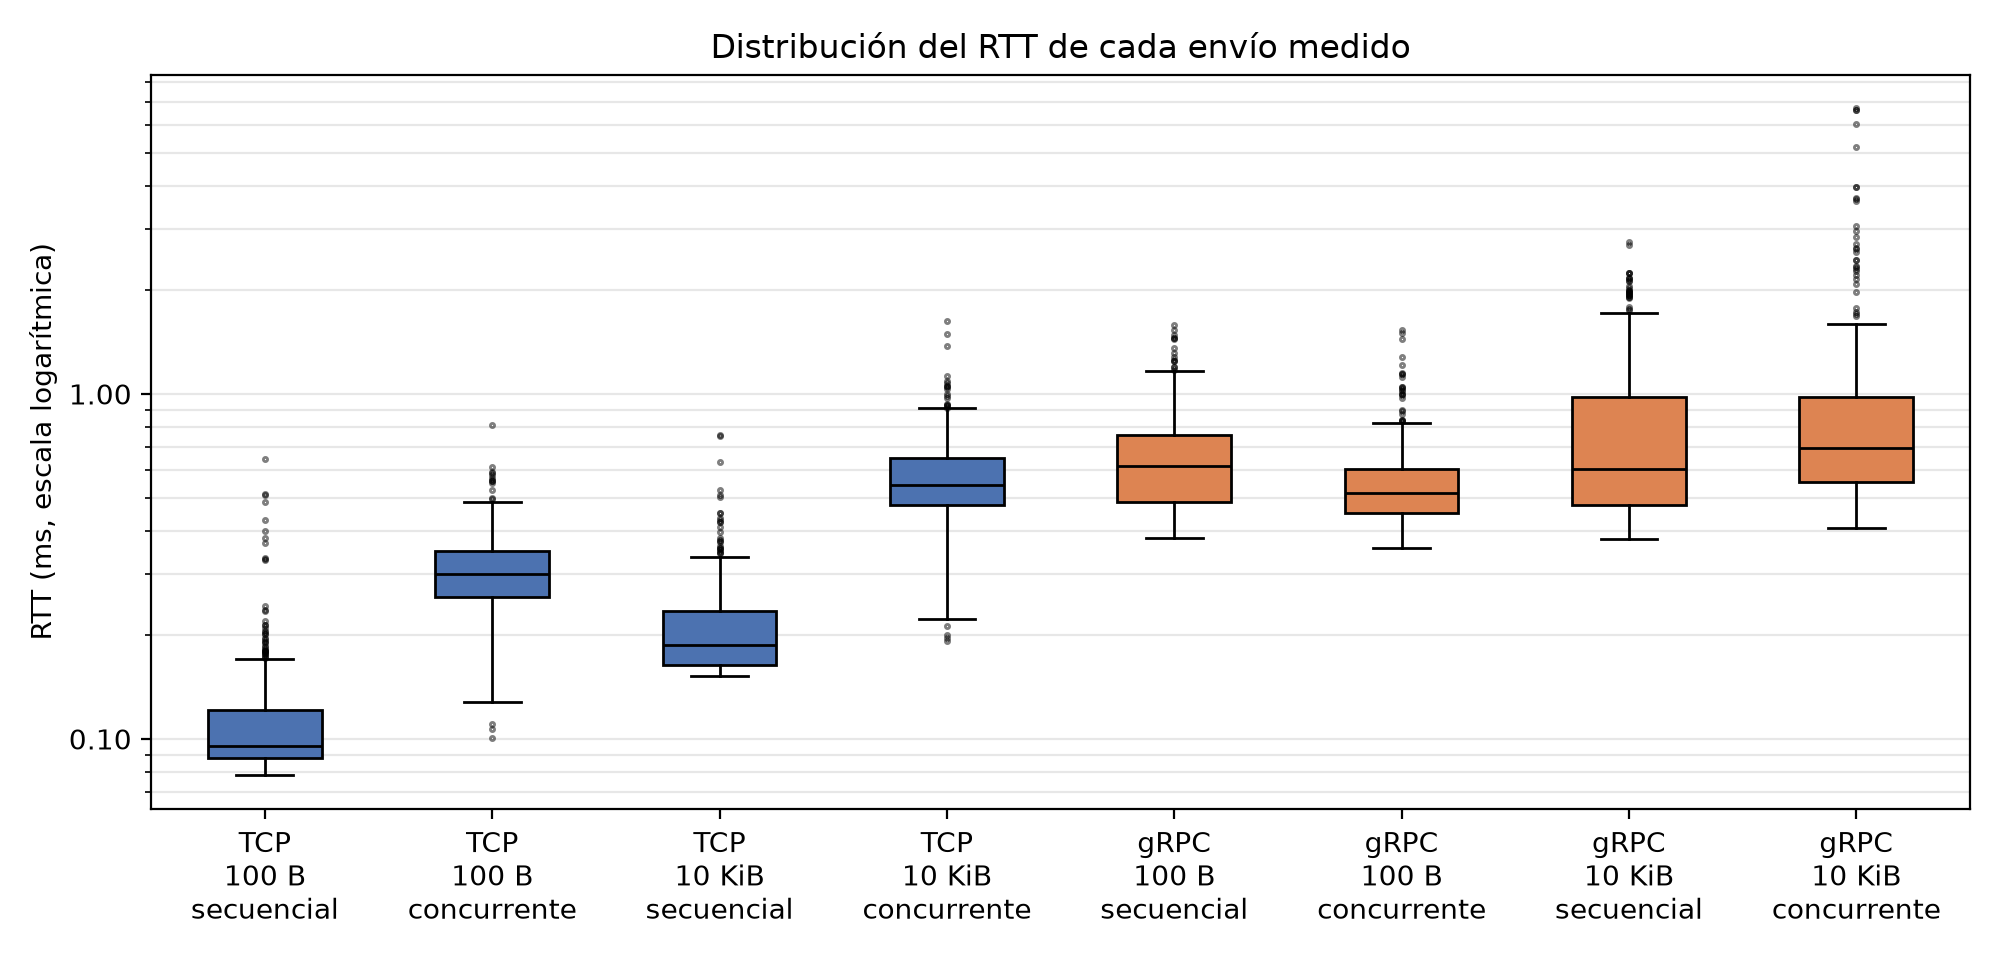
\includegraphics[width=\textwidth]{../analysis/resultados/grafico_cajas.png}
\caption{Distribución del RTT por mecanismo, carga y modo}
\label{fig:cajas}
\end{figure}

\begin{figure}[htbp]
\centering
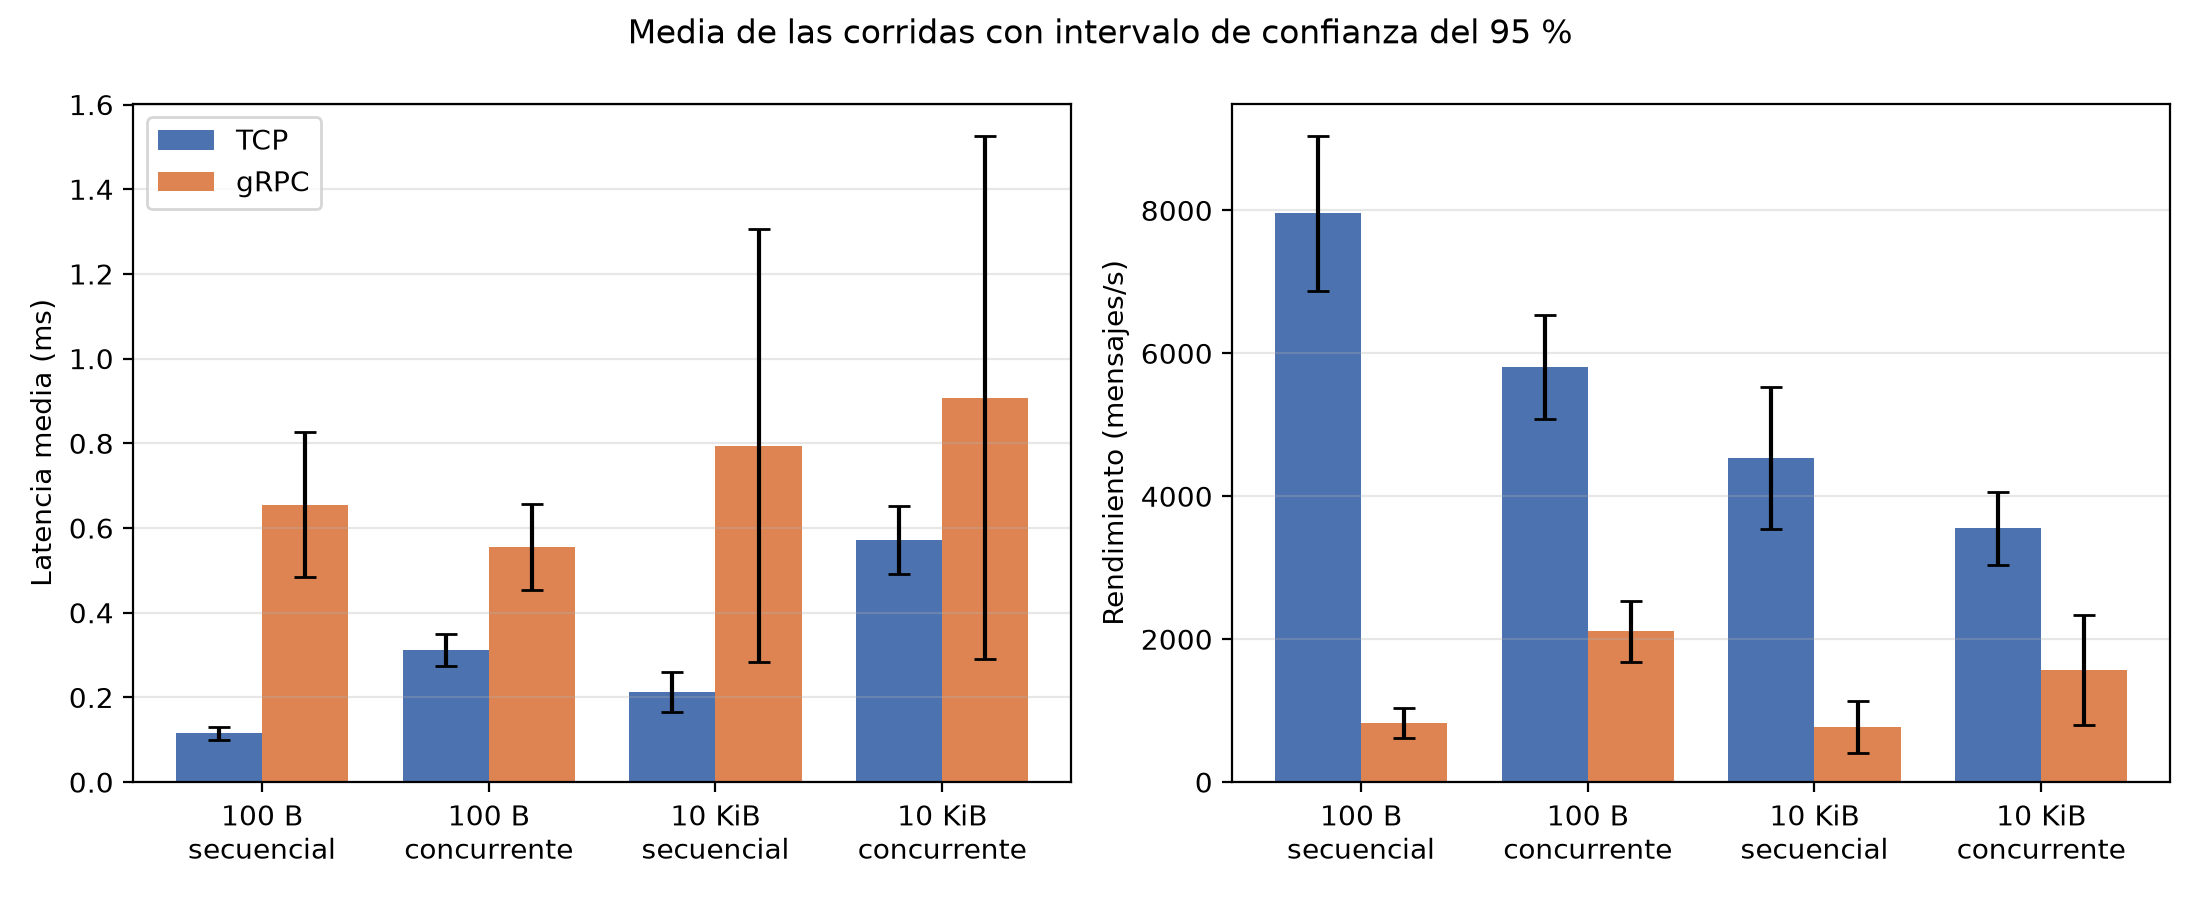
\includegraphics[width=\textwidth]{../analysis/resultados/grafico_barras.png}
\caption{Latencia media y rendimiento con intervalo de confianza del 95~\%}
\label{fig:barras}
\end{figure}


\section{Discusión}
% Aporte de Darwin Joel Sánchez Vera.
\subsection{Discusión de latencia y rendimiento}

TCP obtuvo menor latencia en las cuatro condiciones. La diferencia más grande apareció con mensajes de 100~B en modo secuencial: la mediana fue de 0,0953~ms con TCP y de 0,6171~ms con gRPC, es decir, gRPC tuvo una mediana 547,6~\% mayor. En modo concurrente con 10~KiB la diferencia de la mediana bajó a 27,9~\%, aunque el percentil 95 de gRPC siguió siendo 145,4~\% mayor que el de TCP. En la figura~\ref{fig:barras} los intervalos de la latencia media de TCP y gRPC no se superponen en tres condiciones. Solo se superponen con 10~KiB en modo concurrente, por lo que en esa condición la diferencia de medias es menos concluyente que la de medianas.

El tamaño del mensaje afectó de forma distinta a cada mecanismo. En modo secuencial, al pasar de 100~B a 10~KiB la mediana de TCP subió de 0,0953 a 0,1869~ms (96~\% más), mientras que la de gRPC pasó de 0,6171 a 0,6054~ms. Con nuestras implementaciones, el costo de gRPC parece depender poco de la carga en ese rango y mucho del trabajo fijo de cada llamada; en TCP, en cambio, codificar y copiar el JSON crece con el mensaje. No medimos por separado la serialización, así que esta explicación queda como hipótesis a comprobar.

La concurrencia también tuvo efectos opuestos. En TCP, enviar desde los tres nodos a la vez elevó la mediana con 100~B de 0,0953 a 0,3014~ms. Los tres nodos de TCP comparten un solo proceso, lo que puede explicar parte de ese aumento. En gRPC la mediana concurrente fue menor que la secuencial (0,5166 frente a 0,6171~ms con 100~B); nuestras mediciones no permiten aislar la causa de ese comportamiento.

El rendimiento de gRPC fue entre 55,9~\% y 89,6~\% menor que el de TCP. Esta comparación no es tan directa como la del RTT. En gRPC, la duración de la tanda incluye, por cada envío, la llamada del lanzador al servicio \texttt{ControlNodo.Intercambiar}, que no forma parte del RTT medido. Con 100~B en modo secuencial, cada envío de gRPC ocupó en promedio 1,21~ms de la tanda ($1/825{,}6$~s), aunque su RTT medio fue de 0,655~ms; en TCP la diferencia equivalente fue de 0,126 frente a 0,115~ms. Esto es coherente con que el rendimiento de gRPC suba en modo concurrente (2\,112,9 frente a 825,6~mensajes/s), donde las tres llamadas de control se solapan.

La variación entre corridas fue mayor en gRPC con 10~KiB. Las corridas de la repetición 2 de esas dos combinaciones, ejecutadas una tras otra en las posiciones 22 y 23 de la sesión, tuvieron medias de 1,49 y 1,77~ms, frente a valores entre 0,48 y 0,83~ms en las demás repeticiones. Esas dos corridas amplían el intervalo de confianza de la figura~\ref{fig:barras}. Las conservamos porque son mediciones válidas y el protocolo no prevé descartar corridas por su valor.

En la hipótesis planteamos que TCP tendría menor mediana con 100~B y que con 10~KiB la serialización podría cambiar la diferencia. La primera parte se cumplió. La segunda se cumplió parcialmente: con 10~KiB la diferencia relativa de la mediana bajó de 547,6~\% a 224,0~\% en modo secuencial y de 71,4~\% a 27,9~\% en modo concurrente, pero TCP mantuvo la menor mediana en todas las condiciones.

% Aporte de Darwin Joel Sánchez Vera.
\subsection{Amenazas a la validez}
\label{sec:amenazas}

Identificamos los siguientes factores que pudieron distorsionar las mediciones:

\begin{itemize}
\item \textbf{Una sola máquina y sin red física.} Los nodos se comunicaron por la interfaz \texttt{127.0.0.1}, así que el RTT no incluye la latencia de una red real y los procesos compitieron por el mismo procesador. En una red local o en contenedores separados, la diferencia entre ambos mecanismos podría ser otra.
\item \textbf{Distinta forma de ejecutar los nodos.} TCP ejecutó los tres nodos como hilos de un solo proceso, mientras que gRPC usó tres procesos. En TCP los nodos comparten el bloqueo global del intérprete de Python, lo que afecta sobre todo al modo concurrente. En gRPC cada envío cruza procesos distintos.
\item \textbf{Rendimiento de gRPC medido con el canal de control.} La duración de una tanda gRPC incluye una llamada de control por cada envío. Por eso el rendimiento de gRPC está subestimado frente al de TCP. El RTT no tiene este problema, porque ambos lo miden en el nodo emisor alrededor de un único intercambio.
\item \textbf{Ruido del sistema operativo.} Las corridas 22 y 23 de la sesión, ambas de gRPC con 10~KiB, tuvieron medias de RTT de más del doble que las demás repeticiones de su combinación. No registramos la carga de la máquina durante la sesión, por lo que no podemos atribuir esa variación a un programa concreto. El orden rotado de las combinaciones reparte este efecto entre mecanismos, pero no lo elimina.
\item \textbf{Una sola sesión y un solo equipo.} Las 40 corridas medidas pertenecen a una sesión de unos dos minutos en un equipo con el plan de energía ``Equilibrado''. Incluso dentro de esa sesión, la media de TCP con 10~KiB secuencial varió entre 0,178 y 0,255~ms de una corrida a otra. Los valores absolutos deben leerse como propios de este entorno; otra sesión u otro equipo pueden dar valores distintos.
\item \textbf{Primer envío de cada corrida.} El calentamiento descarta la primera corrida completa, pero dentro de cada corrida medida el primer envío sigue siendo más lento: en las ocho combinaciones, la mediana del primer envío de las corridas superó a la del resto de envíos. Lo conservamos porque el protocolo no descarta envíos individuales; su peso es de un envío por cada 100.
\item \textbf{Implementaciones propias.} Comparamos nuestro cliente TCP con JSON y nuestro servicio gRPC con Protocol Buffers, no los mecanismos en abstracto. Otra codificación en TCP o una configuración distinta de gRPC, por ejemplo con flujos o con otro tamaño de grupo de hilos, podría cambiar los resultados.
\end{itemize}

\subsection{Aplicación al PFC de gestión de pre-sustentaciones}

En el PFC del equipo BCCP desarrollamos un sistema de gestión de
documentos de pre-sustentaciones de trabajos de titulación. En la
arquitectura del proyecto, el servicio de Evaluación y actas necesita
consultar al de Solicitudes y documentos antes de habilitar la rúbrica
para el tribunal~\cite{pfcBccpComunicacion}.

\paragraph{gRPC para consultar una solicitud.}
En el esqueleto del PFC, Evaluación llama al método
\texttt{ConsultarSolicitud} con el identificador de la solicitud.
Solicitudes devuelve su estado, si el informe y el reporte de URKUND
están cargados y el porcentaje de coincidencia. Usamos gRPC porque
Evaluación necesita una respuesta síncrona y un contrato que fije los
tipos de esos campos. El cliente espera hasta cinco segundos y
comunica el estado de error si falla la consulta. En el flujo previsto,
sin esos datos confirmados, Evaluación no habilita la
rúbrica~\cite{pfcBccpRepositorio,pfcBccpComunicacion}.

\paragraph{Sockets TCP para un diagnóstico interno.}
Como extensión de la práctica, proponemos una prueba de conectividad
desde el entorno de Evaluación hacia el puerto \(50051\) de Solicitudes,
que es el puerto del esqueleto local~\cite{pfcBccpRepositorio}.
Un cliente de diagnóstico podría abrir un socket TCP con un tiempo de
espera y registrar si la conexión se estableció, fue rechazada o expiró.
Ese resultado ayudaría a distinguir un problema de conectividad de un
error devuelto por la llamada gRPC. Una conexión establecida indica que
el puerto acepta conexiones. Para comprobar que el trámite puede
consultarse correctamente, necesitamos ejecutar la llamada gRPC.

\section{Verificación del reloj de Lamport}


\subsection{Método}
El script \texttt{analysis/verificar\_lamport.py} lee los CSV de eventos reales
de \texttt{data/} y analiza cada corrida por separado. Cada envío
(\texttt{send}) se empareja con su recepción (\texttt{receive}) cuando
coinciden el identificador de corrida (\texttt{run\_id}), el identificador de
mensaje (\texttt{message\_id}) y el tipo (\texttt{request} o
\texttt{response}), y el nodo emisor es el par del receptor. En cada par se
comprueba que $L(\text{recepción}) > L(\text{envío})$.

Para analizar la concurrencia, el script reconstruye la relación
\emph{ocurrió antes} ($\rightarrow$) definida por Lamport~\cite{lamport1978}:
dentro de un nodo, cada evento ocurre antes que el siguiente, y el envío de un
mensaje ocurre antes que su recepción. Dos eventos $a$ y $b$ son concurrentes
($a \parallel b$) si no se cumple $a \rightarrow b$ ni $b \rightarrow a$.

\subsection{Resultados}
La Tabla~\ref{tab:lamport} resume las 40 corridas medidas de la sesión
oficial. La columna \emph{Mensajes} cuenta por separado la solicitud y la
respuesta de cada envío, por lo que cada corrida de 100 envíos aporta 200
mensajes. En todas las combinaciones, el reloj de recepción fue mayor que el
de envío en todos los mensajes, y no quedó ningún evento sin pareja. El script
también verifica las corridas de calentamiento y las pruebas previas; sus
resultados quedan en \texttt{analysis/resultados/lamport\_por\_archivo.csv}.

\begin{table}[ht]
\centering
\caption{Verificación de Lamport en la sesión oficial (generada por el script).
\emph{Iguales y conc.}: pares de eventos de nodos distintos con el mismo reloj
que son concurrentes.}
\label{tab:lamport}
\resizebox{\textwidth}{!}{\begin{tabular}{llrrrrr}
\toprule
Conjunto & Mecanismo & Eventos & Mensajes & Cumplen & Fallan & Iguales conc. \\
\midrule
demo\_grpc & gRPC & 60 & 30 & 30 & 0 & 2 \\
tcp\_20\_100b\_eventos & TCP & 80 & 40 & 40 & 0 & 19 \\
tcp\_20\_10kib\_eventos & TCP & 80 & 40 & 40 & 0 & 19 \\
tcp\_concurrente\_10kib\_eventos & TCP & 84 & 42 & 42 & 0 & 68 \\
\bottomrule
\end{tabular}
}
\end{table}

\subsection{Eventos concurrentes con el mismo reloj}
La Tabla~\ref{tab:concurrentes} muestra un ejemplo real por mecanismo y modo.
En el modo concurrente, nodo-A y nodo-B envían su primera solicitud con
$L=1$: ninguno había recibido nada, así que ninguno pudo influir en el otro.
En el modo secuencial, nodo-A recibe la respuesta del mensaje 0001 con $L=4$
al mismo valor con que nodo-B envía la solicitud 0002, y tampoco existe una
cadena de mensajes que conecte esos dos eventos.

\begin{table}[ht]
\centering
\caption{Ejemplos de eventos concurrentes con igual reloj (generada por el script).}
\label{tab:concurrentes}
\resizebox{\textwidth}{!}{\begin{tabular}{lrll}
\toprule
Conjunto & Reloj & Evento 1 & Evento 2 \\
\midrule
demo\_grpc & 20 & nodo-A receive response 0005 & nodo-B send request 0001 \\
tcp\_20\_100b\_eventos & 4 & nodo-A receive response 0001 & nodo-B send request 0002 \\
tcp\_20\_10kib\_eventos & 4 & nodo-A receive response 0001 & nodo-B send request 0002 \\
tcp\_concurrente\_10kib\_eventos & 1 & nodo-A send request 0001 & nodo-B send request 0002 \\
\bottomrule
\end{tabular}
}
\end{table}

\subsection{Por qué Lamport no distingue este caso}
El reloj de Lamport solo garantiza la condición
$a \rightarrow b \Rightarrow L(a) < L(b)$; la implicación inversa no se cumple.
Por eso, dos relojes iguales indican que los eventos no tienen relación causal,
pero un reloj menor no indica que un evento haya causado al otro. Los datos lo
confirman: el script encontró pares de eventos con relojes distintos que también
son concurrentes (columna \texttt{reloj\_distinto\_concurrentes} de
\texttt{lamport\_resumen.csv}). Con un solo número por evento no se puede saber
si dos eventos son concurrentes; para eso se necesitan relojes vectoriales, que
guardan un contador por cada nodo.

\section{Conclusiones}

% Todas las cifras salen de las tablas generadas por los scripts.

\begin{itemize}
  \item TCP obtuvo menor latencia que gRPC en las cuatro condiciones medidas.
  Con mensajes de 100~B en modo secuencial, la mediana del RTT de gRPC fue
  547,6~\% mayor que la de TCP (0,6171~ms frente a 0,0953~ms).
  \item La diferencia se redujo con mensajes grandes y con concurrencia: con
  10~KiB en modo concurrente, la mediana de gRPC fue solo 27,9~\% mayor, aunque
  su percentil~95 siguió siendo 145,4~\% mayor que el de TCP.
  \item El rendimiento de gRPC fue entre 55,9~\% y 89,6~\% menor que el de TCP,
  con la salvedad de que la duración de las tandas de gRPC incluye la llamada
  de control de cada envío.
  \item La hipótesis se cumplió en la parte de mensajes cortos; con 10~KiB la
  diferencia bajó, pero TCP mantuvo la menor mediana en todos los casos.
  \item En los 8\,000 mensajes de las 40 corridas medidas, el reloj de Lamport
  al recibir fue mayor que al enviar en el 100~\% de los casos, y el script
  encontró pares de eventos concurrentes con el mismo reloj, lo que confirma
  que Lamport no basta para detectar la concurrencia.
\end{itemize}

\section{Tabla de aportes}

La Tabla~\ref{tab:aportes} resume el trabajo de cada integrante. El enlace
muestra todos sus commits en el repositorio.

\begin{table}[ht]
\centering
\caption{Aportes de cada integrante.}
\label{tab:aportes}
\small
\begin{tabular}{@{}p{3.3cm}p{8.4cm}p{3.3cm}@{}}
\toprule
Integrante & Aporte & Commits \tabularnewline
\midrule
\raggedright Jilmar Jesús Cedeño Intriago &
\raggedright Servidor y clientes con sockets TCP (\texttt{src/sockets/}), reloj de Lamport
en TCP, corridas TCP, sección de implementación TCP y aplicación al PFC. &
\href{https://github.com/jcedenoi4/GA-SUM-02/commits?author=jcedenoi4}{\texttt{jcedenoi4}} \tabularnewline
\addlinespace
\raggedright Angello Agustín Mendoza Bermello &
\raggedright Contrato \texttt{proto/lamport.proto}, nodos gRPC (\texttt{src/grpc/}), reloj
de Lamport en gRPC, demostración con capturas y sección de implementación gRPC. &
\href{https://github.com/jcedenoi4/GA-SUM-02/commits?author=Amendozab5}{\texttt{Amendozab5}} \tabularnewline
\addlinespace
\raggedright Darwin Joel Sánchez Vera &
\raggedright Protocolo experimental (\texttt{analysis/ejecutar\_protocolo.py}), análisis
estadístico y gráficos (\texttt{analysis/estadisticas.py}), \texttt{SHA256SUMS},
secciones de protocolo, resultados, discusión y amenazas a la validez. &
\href{https://github.com/jcedenoi4/GA-SUM-02/commits?author=DarwinDevCode}{\texttt{DarwinDevCode}} \tabularnewline
\addlinespace
\raggedright Leonel Leonidas Zambrano Triviño &
\raggedright Verificador de Lamport (\texttt{analysis/verificar\_lamport.py}), diagrama de
arquitectura, sección de verificación de Lamport, integración del informe,
\texttt{README.md} y bitácora. &
\href{https://github.com/jcedenoi4/GA-SUM-02/commits?author=lzambranot6-sys}{\texttt{lzambranot6-sys}} \tabularnewline
\bottomrule
\end{tabular}
\end{table}

\section{Declaración de uso de inteligencia artificial}

Declaramos el uso de herramientas de inteligencia artificial generativa en las
siguientes partes del trabajo. Todo el contenido fue revisado, ejecutado y
verificado por el equipo, y cada integrante puede explicar su parte.

\begin{itemize}
  \item \textbf{Leonel Zambrano:} usó Claude (Anthropic) como apoyo para
  estructurar el script de verificación de Lamport
  (\texttt{analysis/verificar\_lamport.py}), el diagrama
  de arquitectura en TikZ y la estructura de su sección del informe. Revisó y
  ejecutó el código con los datos reales y reescribió el texto.
  \item \textbf{Jilmar Cedeño:} % completar
  \item \textbf{Angello Mendoza:} % completar (en el chat mencionaron Codex)
  \item \textbf{Darwin Sánchez:} % completar
\end{itemize}

Las cifras, tablas y gráficos provienen de la ejecución real de los scripts
del repositorio sobre los CSV de \texttt{data/}; ninguna medición fue generada
por una herramienta de IA.


\printbibliography
\end{document}
